% !TEX TS-program = pdflatex
% !TEX encoding = UTF-8 Unicode

% This is a simple template for a LaTeX document using the "article" class.
% See "book", "report", "letter" for other types of document.

\documentclass[11pt]{article} % use larger type; default would be 10pt

%\usepackage[utf8]{inputenc} % set input encoding (not needed with XeLaTeX)

%%% Examples of Article customizations
% These packages are optional, depending whether you want the features they provide.
% See the LaTeX Companion or other references for full information.

%%% PAGE DIMENSIONS

\usepackage{geometry} % to change the page dimensions
\geometry{a4paper} % or letterpaper (US) or a5paper or....
%\geometry{margins=2in} % for example, change the margins to 2 inches all round
% \geometry{landscape} % set up the page for landscape
%   read geometry.pdf for detailed page layout information
\usepackage{fullpage}
%\usepackage[top=tlength, bottom=blength, left=llength, right=rlength]{geometry}
%Edit individual page dimension variables described above, using the \addtolength and \setlength commands. For instance,
%\oddsidemargin=-1cm
%\setlength{\textwidth}{6.5in}
%\addtolength{\voffset}{-5pt}

\usepackage{graphicx} % support the \includegraphics command and options

% \usepackage[parfill]{parskip} % Activate to begin paragraphs with an empty line rather than an indent

%%% PACKAGES
\usepackage{booktabs} % for much better looking tables
\usepackage{array} % for better arrays (eg matrices) in maths
\usepackage{paralist} % very flexible & customisable lists (eg. enumerate/itemize, etc.)
\usepackage{verbatim} % adds environment for commenting out blocks of text & for better verbatim
%\usepackage{subfig} % make it possible to include more than one captioned figure/table in a single float

\usepackage{caption}
\usepackage{subcaption}
\usepackage{cite}
\usepackage{graphicx}
\usepackage{hyperref, amsmath, mathrsfs, bm}

\usepackage{url}
\renewcommand{\thesubfigure}{}
% justifying
\usepackage{ragged2e}


\graphicspath{{./}{./../graphs/}{./graphs/}}


\usepackage{amssymb,amsmath,amsthm,amscd}

\usepackage[mathscr]{eucal}
%\usepackage[dvips]{graphicx}
%\usepackage{pstricks,pst-grad,pst-plot,pst-node}


%\usepackage{pgf}



%\newpsobject{showgrid}{psgrid}{subgriddiv=1,griddots=2,gridlabels=6pt}
\renewcommand{\raggedright}{\leftskip=0pt \rightskip=0pt plus 0cm}
% argmin
\DeclareMathOperator*{\argmin}{arg\,min}

\newcommand{\myred}{\color{red}}
\newcommand{\mygreen}{\color{green!50!black}}
\newcommand{\myblue}{\color{blue}}

\newcommand{\mcX}{\mathcal{X}}
\newcommand{\mcY}{\mathcal{Y}}
\newcommand{\mcG}{\mathcal{G}}
\newcommand{\mcF}{\mathcal{F}}


%\usepackage[tiling]{pst-fill}
\usepackage{epsfig}
\usepackage{graphicx}
\usepackage[usenames,dvipsnames]{color}

\usepackage{Sweave}
\usepackage{tikz}
\usepackage{pgf}

%%% HEADERS & FOOTERS
\usepackage{fancyhdr} % This should be set AFTER setting up the page geometry
\pagestyle{fancy} % options: empty , plain , fancy
\renewcommand{\headrulewidth}{0pt} % customise the layout...
\lhead{}\chead{}\rhead{}
\lfoot{}\cfoot{\thepage}\rfoot{}

%%% SECTION TITLE APPEARANCE
%\usepackage{sectsty}
%\allsectionsfont{\sffamily\mdseries\upshape} % (See the fntguide.pdf for font help)
% (This matches ConTeXt defaults)

%%% ToC (table of contents) APPEARANCE
\usepackage[nottoc,notlof,notlot]{tocbibind} % Put the bibliography in the ToC
\usepackage[titles,subfigure]{tocloft} % Alter the style of the Table of Contents
\renewcommand{\cftsecfont}{\rmfamily\mdseries\upshape}
\renewcommand{\cftsecpagefont}{\rmfamily\mdseries\upshape} % No bold!

\newtheorem{thm}{Theorem}
\newtheorem{cor}{Corollary}
\newtheorem{lem}{Lemma}





%%% END Article customizations

%%% The "real" document content comes below...

\title{ Fidelity-Commensurability Tradeoff in Joint Embedding of Disparate Dissimilarities}


%input affiliations


\author{Sancar Adali\thanks{Johns Hopkins University,
Department of Applied Mathematics and Statistics,
100 Whitehead Hall,
3400 North Charles Street,
Baltimore, MD 21218-2682} \and Carey E. Priebe\thanks{Johns Hopkins University,
Department of Applied Mathematics and Statistics,
100 Whitehead Hall,
3400 North Charles Street,
Baltimore, MD 21218-2682}
}
 

% \email{sadali1@jhu.edu}   %optional

% \email{cep@jhu.edu}   %optional
\date {August 1, 2011}% Activate to display a given date or no date (if empty),
         % otherwise the current date is printed 

\begin{document}
\maketitle
\abstract{For matched data from disparate sources (objects observed under different conditions), optimality of information fusion must be defined with respect to the inference task at hand. Defining the task as matched/unmatched hypothesis testing for dissimilarity observations,  Priebe et al.~\cite{JOFC} presents manifold matching using an embedding method based on joint optimization of fidelity (preservation of within-condition dissimilarities between observations of an object) and commensurability (preservation of between-condition dissimilarities between observations) . The tradeoff between fidelity and commensurability is investigated by varying weights in weighted embedding of an omnibus dissimilarity matrix. Optimal (defined with respect to the power of the test) weights for the optimization correspond to an optimal compromise between fidelity and commensurability. Results indicate optimal weights are different than equal weights for commensurability and fidelity and the proposed weighted embedding scheme provides significant improvements in test power.
}




\section{Introduction}

 It is a challenge  to do a tractable analysis on data from disparate sources of data (such as multiple sensors). The multitude  of sensors technology and large numbers of sensors both are  sources of difficulty and hold promise for efficient inference.
 \begin{comment}
 The typical multiple sensor setting is visualized in  Figure ~\ref{fig:fig1}.
\begin{figure}
\centering
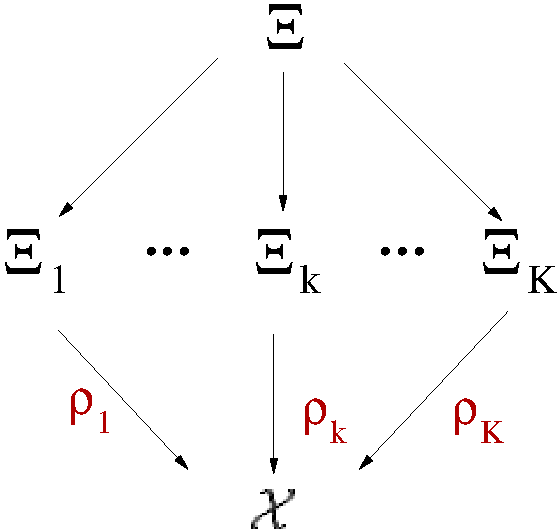
\includegraphics[scale=0.75]{gen-model-orig-proj.pdf}
\caption{Multiple Sensor setting}
\label{fig:fig1}
\end{figure}
\end{comment}


In the problem setting considered, $n$ different objects/instances are measured/judged under $K$ different conditions (corresponding possibly to $K$ different sensors) using  dissimilarity measures. These will be represented in matrix form as $K$ $n \times n$ matrices $\{\Delta_k,k=1 ,\ldots,K\}$.  In addition,  dissimilarities between  $K$ new measurements/observations  and the previous 
$n$ objects under $K$ conditions are given. The inference task is to    test the null hypothesis  that ``these measurements are from the same  object"  (matched) against the alternative hypothesis that ``they are not  from the same  object" (unmatched)~\cite{JOFC}:
  In order to get a data representation where dissimilarities from disparate sources can be compared, the dissimilarities must be mapped to a commensurate metric space where the metric can be used to distinguish between ``matched" and ``unmatched" pairs.


To embed dissimilarities  $\{\Delta_k,k=1 ,\ldots,K\}$  from different conditions into a commensurate space in one step, an omnibus dissimilarity matrix  $M$ can be embedded in the low-dimensional Euclidean space , imputing entries if necessary. Consider, for $K=2$ \footnote{Throughout this paper , it will be assumed,  the number of conditions, $K$, is equal to $2$ for the  simplicity of presentation. The approaches are easily generalizable to $K>2$ conditions.},
 \begin{equation}
M=  \left[ \begin{array}{cc}
         \Delta_1 & L\\
        L^T  & \Delta_2 
     \end{array}  \right]     \label{omnibus} 
\end{equation} where $L$ is a matrix of imputed entries. Using MDS to embed  this omnibus matrix into a  commensurate space  ,  $2n$ embedded observations $\{\tilde{y}_i^{(k)}; i=1,\ldots,n;k=1,2\}$ are obtained. \footnote{ 
It  will be assumed  the commensurate space  $\mathcal{X}$  is  $\mathbb{R}^d$ where $d$ is pre-specified. The selection of $d$ -- model selection -- is  a task that requires much attention and is  beyond the scope of this article. Discussion of the effect of $d$ on matching performance will be available at a later paper.  }, with distances between the different observations consistent with the given dissimilarities. Now that the observations are commensurate, it is possible to  compute the test statistic \[
\tau=d\left(\tilde{y}_i^{(1)},\tilde{y}_j^{(2)}\right)\label{teststat}
\] for $i^{th}$ and $j^{th}$ observations under different conditions.  For ``large" values of $\tau$, the null hypothesis will be rejected. This approach will be referred to as the Joint Optimization of Fidelity and Commensurability (JOFC) approach, for reasons that will be explained. 
  Out-of-sample extension for MDS will be used throughout this paper\cite{TrossetOOS}. 


Regardless of the inference task,  to expect reasonable performance from the embedded data in the commensurate space, two criteria must be adhered to:

\begin{itemize}
\item Fidelity is how well the mapping to commensurate space preserves the original dissimilarities. The loss of \em{fidelity} can be measured with  within-condition \em{ infidelity error} is given by
    \[
\epsilon_{f_{k}} = \frac{1}{{{n}\choose{2}}} \sum_{1 \leq i < j \leq n} (d(\widetilde{\bm{x}}_{ik},\widetilde{\bm{x}}_{jk})-\delta_{ijk})^2
\] 
where $\delta_{ijk}$ is the dissimilarity between $i^{th}$ object and $j^{th}$ object where both objects are in the $k^{th}$  condition and $\widetilde{\bm{x}}_{ik}$ is the embedded configuration of the $i^{th}$ object  for the $k^{th}$ condition;  $d(\cdot,\cdot)$ is the Euclidean distance function (for the embedding space).

\item Commensurability is how well the mapping to commensurate space preserves matchedness of matched observations. The loss of commensurability can be measured by the between-condition {\em incommensurability error} which is given by
    \[
\epsilon_{c_{k_1k_2}} = \frac{1}{n} \sum_{1 \leq i \leq n;k_1 <k_2} (d(\widetilde{\bm{x}}_{ik_1},\widetilde{\bm{x}}_{ik_2})- { \delta_{ijk_1k_2}})^2
\label{comm-error}
\]
 for conditions $k_1$ and $k_2$; $\delta_{ijk_1k_2}$  is the dissimilarity between $i^{th}$ object under  $k_1^{th}$ condition  and $j^{th}$ object under $k_2^{th}$ condition.
\end{itemize}

While  \emph{infidelity} and  \emph{incommensurability} errors as measured by the above expressions is specific to the joint embedding scheme by MDS, the concepts of fidelity and commensurability are  general enough to be applicable to other dimensionality reduction methods that can be used on data from disparate sources.



The joint embedding results in the joint optimization of fidelity and commensurability and this relation can be made explicit by the use of the raw stress function in MDS embedding. Denoting  $(s,t)^{th}$ entry of $M$ by $M_{st}$ ,
\begin{equation}
\sigma_{W}(\widetilde{X})=\sum_{1\leq s\leq n;1\leq t\leq n} {w_{st}(d_{st}(\widetilde{X})-M_{st})^2  }\label{raw-stress}
\end{equation}

is the MDS criterion function , where individual terms in the sum can be ascribed to fidelity and commensurability respectively. %\footnote{\delta_{ijk_1k_2} is just a reindexing of M_{st}, k_1,k_2 are row/column indices of the block matrix (i,j)  are  row/column indices of the matrix entry, },

\begin{comment}
\begin{align}
\sigma_W(\cdot)  &= & &\sum_{i,j,k_1,k_2} {w_{ij{k_1}{k_2}}(d_{ij{k_1}{k_2}}(\cdot)-\delta_{ijk_1k_2})^2 }_{term with indices {i,j,k_1,k_2}} \notag\\
\hspace{3pt} &=& &\underbrace{\sum_{i=j,k_1<k_2}  {w_{ij{k_1}{k_2}}(d_{ij{k_1}{k_2}}(\cdot)-\delta_{ijk_1k_2})^2}}_{Commensurability}  \hspace{10pt}  &  + &\hspace{2.5em} \underbrace{\sum_{i<j,k_1=k_2}  {w_{ij{k_1}{k_2}}(d_{ij{k_1}{k_2}}(\cdot)-\delta_{ijk_1k_2})^2  }  } _{Fidelity}\notag\\
\hspace{3pt}&+&  &\underbrace{\sum_{i< j,k_1<k_2}  {w_{ij{k_1}{k_2}}(d_{ij{k_1}{k_2}}(\cdot)-\delta_{ijk_1k_2})^2  }  } _{Separability}\label{eq:FidCommSep}\hspace{10pt} .
\end{align}

\end{comment}

\begin{align}
\sigma_W(\cdot)  &= & &\sum_{i,j,k_1,k_2} \underbrace{{w_{ij{k_1}{k_2}}(d_{ij{k_1}{k_2}}(\cdot)-\delta_{ijk_1k_2})^2 }}_{term_{i,j,k_1,k_2}} \notag\\
\hspace{3pt} &=& &\underbrace{\sum_{i=j,k_1<k_2}  term_{i,j,k_1,k_2}}_{Commensurability}  \hspace{10pt}  &  + &\hspace{2.5em} \underbrace{\sum_{i<j,k_1=k_2}   term_{i,j,k_1,k_2}  } _{Fidelity}
\hspace{3pt}&+&  &\underbrace{\sum_{i< j,k_1<k_2}  term_{i,j,k_1,k_2}  } _{Separability}\label{eq:FidCommSep}\hspace{10pt} .
\end{align}

 The separability error terms will be ignored herein (by setting the associated weights  to be 0), due to the fact that 
$\delta_{k_1k_2}(\bm{x}_{ik_1},\bm{x}_{jk_2})$ is not  available \footnote{Due to the fact that data sources are ``disparate", it is not obvious how  a dissimilarity between an object in one condition and another object in another condition  can be computed or  defined in a sensible way.} and it will be easier to focus on just the fidelity-commensurability tradeoff. Setting $\delta_{ijk_1k_2}$ to 0 \footnote{Although  the between-condition dissimilarities of the same object, ${ \delta_{k_1k_2}(\bm{x}_{ik_1},\bm{x}_{ik_2}})$, are not available,  it is not unreasonable in this setting  to set ${ \delta_{k_1k_2}}(\bm{x}_{ik_1},\bm{x}_{ik_2}) = 0$ for all $i,k_1,k_2$.  So diagonal  entries of $L$ in  equation \eqref{omnibus} are  chosen to be all zeroes. Setting these diagonal entries to zero forces matched points to be embedded close to each other.},
\begin{align}
\sigma_W(\cdot)\hspace{3pt}   
\hspace{3pt}&=&\underbrace{\sum_{i=j,k_1< k_2}  {w_{ij{k_1}{k_2}}(d_{ij{k_1}{k_2}}(\cdot))^2}}_{Commensurability}  \hspace{10pt}  &  +&\underbrace{\sum_{i< j,k_1=k_2}  {w_{ij{k_1}{k_2}}(d_{ij{k_1}{k_2}}(\cdot)-\delta_{ijk_1k_2})^2  }  } _{Fidelity}\notag\label{eq:FidCommSep}\hspace{10pt} .
\end{align}
This motivates  the naming of the   omnibus embedding approach as Joint Optimization of Fidelity and Commensurability (JOFC).

The major question  addressed in this work is whether in the tradeoff between preservation of fidelity and preservation of  commensurability , there is an optimal point for the inference task.  The weights in raw stress allow us to answer this question relatively easily. Setting $w_{ij}$ to $w$ and $1-w$  for commensurability  and fidelity  terms respectively will allow us to control the relative importance of fidelity and commensurability terms in the optimization. 

Previous investigations of JOFC approach assumed unweighted(equivalently, equally weighted) stress functions for MDS embedding. This assumption corresponds to  $w=0.5$ case in this presentation .
The expectation here is that there is a $w^*$   such that  $w^* \neq 0.5$  that is optimal for the specific exploitation task (hypothesis testing, which $w$ value has the best power). That is , the default value of $w=0.5$  is not the ``optimal" value and $w$ should be deliberately chosen.

\begin{comment}
If the source of dissimilarities  are actually observations that are vectors in Euclidean space,  unless 
\begin{itemize}
\item the dissimilarity matrix is the Euclidean distance matrix of the original observations, and, 
\item the embedding dimension is greater or equal to the dimension of the original observations,
\end{itemize}
MDS with raw stress will not result in a perfect reconstruction  of the original observations. Note that the objective of the (joint)embedding is not \emph{perfect} reconstruction, but the best embedding for the exploitation task which is to test whether two sets of dissimilarities are ``matched". What is considered a ``good"'  representation will be dependent on how well the information in original dissimilarities that is relevant to the the match detection task is preserved. Fidelity and commensurability quantify this preservation of information.
\end{comment}

 

\section{``Matched" and ``Conditions" in data}

 ``Conditions" and ``matched" refer to concepts dependent on the context of the  problem. Conditions could be different modalities of data, e.g., one condition could be  an image of an object, while the other condition could be a text description of the object. ``Matched", in general, means observations of the same object, or realizations of a common concept. 
\subsection{Gaussian setting\label{subsec:GaussianSet}}
	Let    $\Xi_1 = \mathbb{R}^{p}$ and $\Xi_2 = \mathbb{R}^{p}$.
  Let $\bm{\alpha}_i \sim^{iid} MVNormal(\bm{0},I_p)$ represent $n$ ``objects".  Let $\bm{x}_{ik}  \sim^{iid} MVNormal(\bm{\alpha_i},\Sigma)$ represent $K=2$ matched measurements (each under a different condition).
  $\Sigma$ is a positive-definite $p\times p$ matrix such that  $\max(\Lambda(\Sigma))=\frac{1}{r} $ where $\Sigma=U\Lambda(\Sigma)U'$  is the eigenvalue decomposition of $\Sigma$. See Figure~\ref{fig:Fig1}.

The parameter $r$ controls the variability between ``matched" measurements. If $r$ is large, it is expected that the distance between matched measurements
$\bm{x}_{i1}$ and $\bm{x}_{i2}$ to be stochastically smaller than $\bm{x}_{i1}$ and $\bm{x}_{i'2}$ for $i \neq i'$ ; if r is small, then ``matched" is not informative in terms of similarity of measurements.
 Smaller $r$ will make the decision problem harder and will lead to higher rate of errors or tests with smaller power for fixed type I error rate $\alpha$.

    \begin{figure}
	\begin{center}
    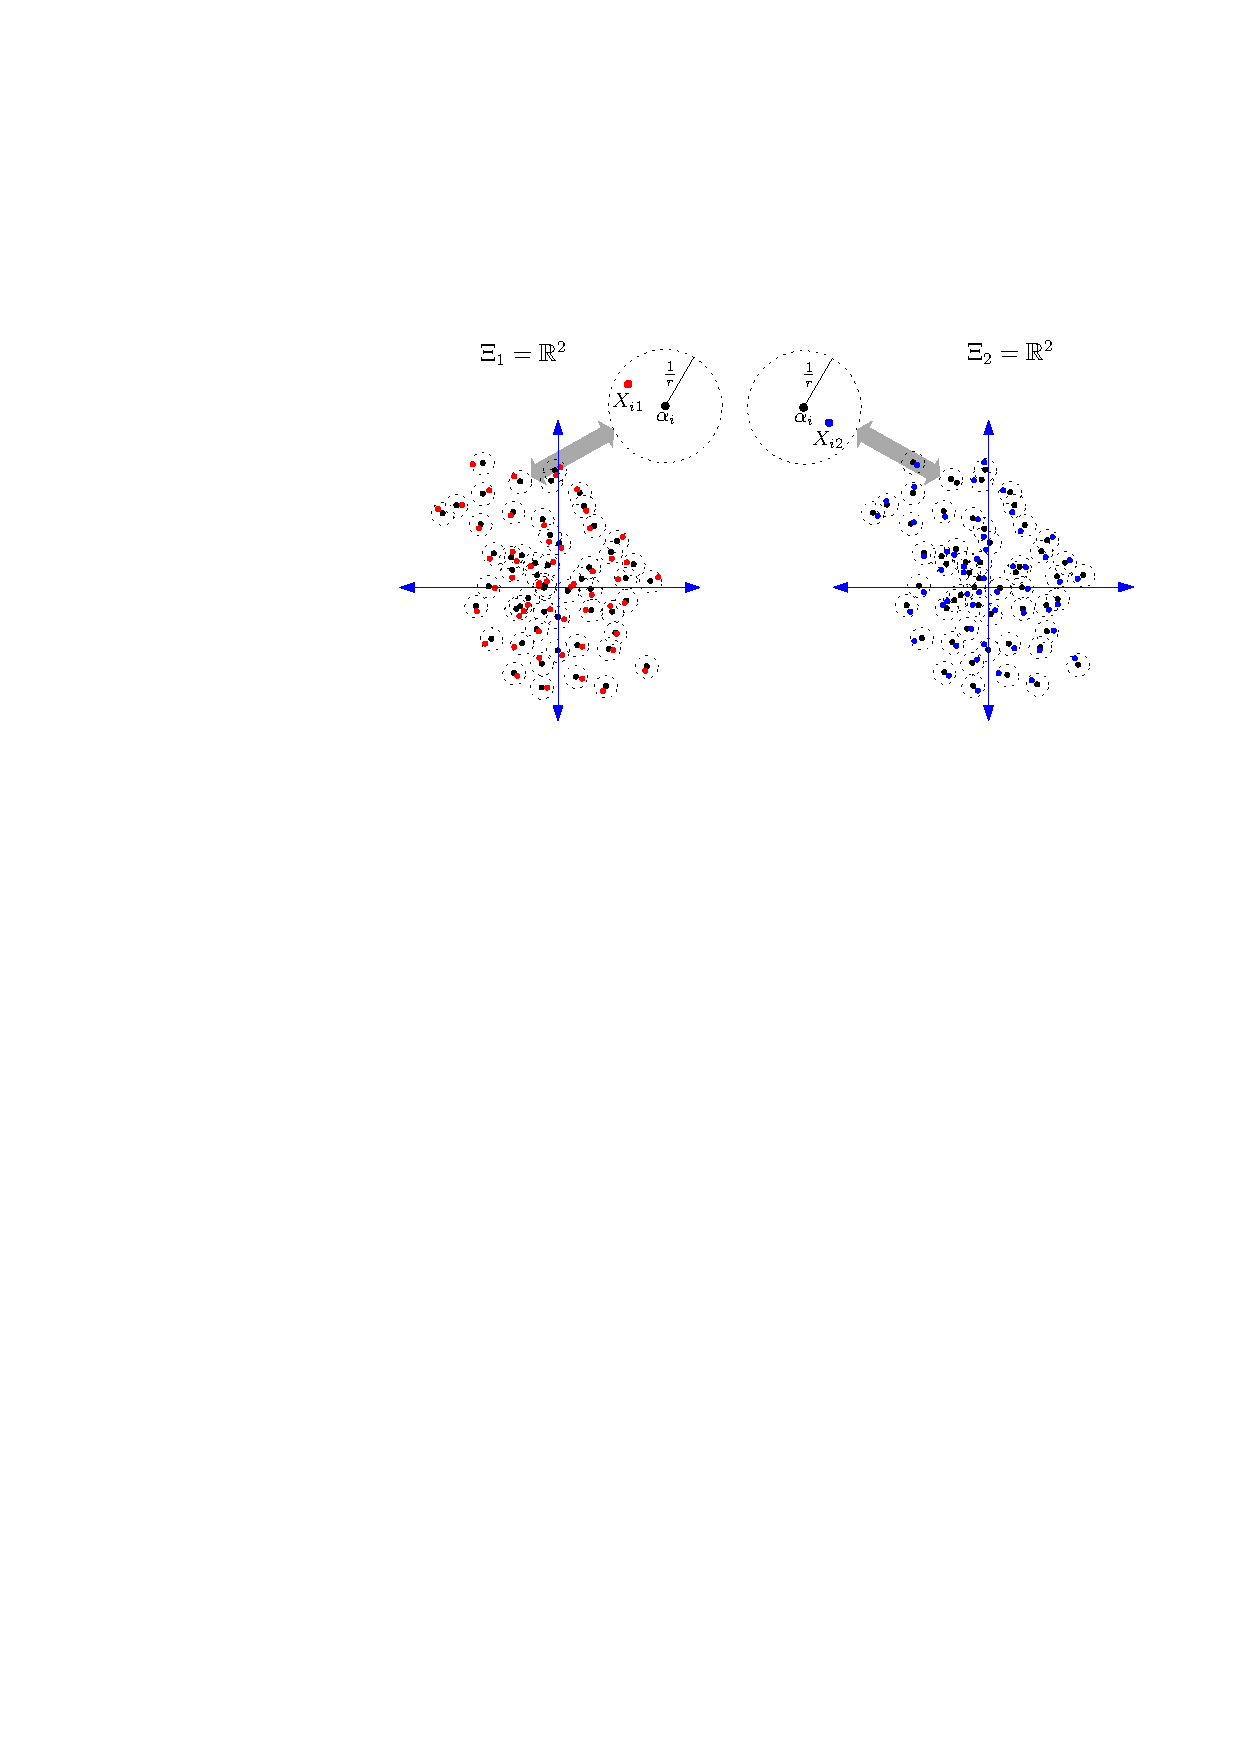
\includegraphics[scale=0.55]{MVN_alpha_r_multiple_sancar.pdf}
    \caption{For the  Gaussian setting (Section \ref{subsec:GaussianSet}), the $\bm{\alpha_i},$ are denoted by black points and the $\bm{x}_{ik}$ are denoted by red and blue points respectively.}
\label{fig:Fig1}
	\end{center}
  \end{figure}

% - given the embedded configuration $X$ of the 
%training observations and the augmented dissimilarity matrix that includes dissimilarities between test observations and %the training observations, and dissimilarities in between the training observations, oos-embedding consists of embedding
%the test points into  the existing configuration so as to be as consistent as possible with these dissimilarities (the distances %between points are as close as possible to the dissimilarities as measured by the criterion function). 


\subsection{Alternative Methodologies}

Two alternative methodologies exist that correspond roughly to the extreme ends of the range of $w$ values ($w \in (0,1)$).
For the optimization of commensurability with fidelity as  secondary priority($w\approx 1$), an alternative method is Canonical Correlational Analysis (CCA)~\cite{Hardoon2004}, which finds optimally correlated projections of two random vectors. For the optimization of fidelity ,  Principal Components Analysis (PCA) finds ``best"' representation separately for two conditions . To optimize commensurability as  secondary priority, one can use the projections computed by PCA to  compute a Procrustes transformation that will make the projections commensurate. This $Procrustes \circ MDS$ approach is  analagous to $w\approx 0$ case for JOFC. 

\section{Related Work \label{sec:RelatedWork}}
There have many efforts toward solving the related problem of ``manifold alignment".``Manifold alignment" seeks to find correspondences between observations from different ``conditions". The setting that is most similar to ours is the semi-supervised setting\cite{Ham}, where a set of correspondences are given and the task is to find correspondences between a new set of points in each condition. In contrast, the hypothesis testing task discussed in this paper is to determine whether any given pair of points is ``matched" or not. The proposed solutions follow a common approach: they look for a common commensurate or a latent space, such that the representations (possibly projections or embeddings) of the observations in the commensurate space match.\cite{Wang2008,Zhai2010,3wayNMDS}


\section{Definition of  $w^{*}$}
Two dissimilarity matrices to be embedded are  $\Delta^{(m)} \left(\left[
\begin{array}{c}
\mathcal{T} \\
X_{1}^{(m)} \\
X_{2}^{(m)} 
\end {array}
\right]
\right)$  and 
 $\Delta^{(u)} \left(\left[
\begin{array}{c}
\mathcal{T}\\
X_{1}^{(u)} \\
X_{2}^{(u)}
\end {array}
\right]\right)$ as two matrix-valued random variables $\Delta^{(m)}:\Omega \rightarrow \mathbf{M}_{(n+2)\times (n+2)} $,$\Delta^{(u)}:\Omega \rightarrow \mathbf{M}_{(n+2)\times (n+2)} $  for the appropriate sample  space $(\Omega)$. $\mathcal{T}$ is i.i.d random sample of ($X_{1}^{(m)},X_{2}^{(m)}$).

 The criterion function for the embedding is $\sigma_W(\cdot) =f_w(D({\cdot}),\Delta)$. All of the random variables following the embedding is dependent on $w$, for the sake of simplicity, it will not be shown in the notation. The embedding for the unmatched pair ${\hat{X}_{1}^{(u)},\hat{X}_{2}^{(u)}}$  is 
 \[
{\hat{X}_{1}^{(u)},\hat{X}_{2}^{(u)}}
=\argmin_{\acute{X}_{1}^{(u)}, \acute{X}_{2}^{(u)}}\left[\min_{\mathbf{\acute{T}}}
{f_w\left(
D\left(
\left[
\begin{array}{c}
\acute{\mathbf{T}} \\
\acute{X}_{1}^{(u)} \\
\acute{X}_{2}^{(u)}
\end {array}
\right]
\right),
\Delta^{(u)}
\right)
}
\right]
\]

A similar expression gives the embedding for the matched pair, where $(u)$ superscript   is replaced by $(m)$.
 Assuming the necessary conditions  for $\hat{X}_{1}^{(m)}$ , $\hat{X}_{2}^{(m)}$ , $\hat{X}_{1}^{(u)}$, $\hat{X}_{2}^{(u)}$ to be random vectors hold, consider the test statistic $\tau=d(\hat{X}_{1}^{\cdot},\hat{X}_{2}^{\cdot})$. Under null hypothesis of matchedness, the distribution of the statistic is governed by the distribution of $\hat{X}_{1}^{(m)}$ and $\hat{X}_{2}^{(m)}$, under the alternative it is governed by  $\hat{X}_{1}^{(u)}$ and $\hat{X}_{2}^{(u)}$.

Denote by $F_Y$ the   cumulative distribution function of  $Y$ where $Y$ can be  any function of $\hat{X}_{k}^{(m)}$ or $\hat{X}_{k}^{(u)}$  for $k=\{1,2\}$ 



 Then $$\beta_{\alpha}\left( w\right)=1-F_{d \left(\hat{X}_{1}^{(u)},\hat{X}_{2}^{(u)}\right)}(F_{d\left(\hat{X}_{1}^{(m)},\hat{X}_{2}^{(m)}\right)}^{-1}(1-\alpha)).$$

 Note that all random variables such as $\hat{X}_{k}^{(m)}$  are dependent on $w$. Finally, define $$w^{*}=\arg\max_w{\beta_{\alpha}\left( w\right)}. $$


Given  specific distributions $\mathbf{F}_{ \hat{X}_{k}^{(m)}}$,$\mathbf{F}_{ \hat{X}_{k}^{(u)}}$,   $w^*$ must be defined with respect to the value of allowable type I error rate $\alpha$.  For two different $\alpha$ values, it is quite possible that $\beta_{\alpha_1}(w_1)>\beta_{\alpha_1}(w_2)$  and $\beta_{\alpha_2}(w_1)<\beta_{\alpha_2}(w_2)$. This can be observed in results in Section \ref{sec:Simulation Results}.  

 $w^*$ is defined to be the argmin of  the power function with respect to $w$ and some important questions about $w^*$ are  related to the nature of this function $\beta_{\alpha}\left( w\right)$.
While finding an analytical expression for the value of $w^*$ is intractable, an estimate $\hat{w}^*$  based on noisy evaluations of $\beta_{\alpha}(w^*)$ can be computed.  A Monte Carlo simulation is run in  Section  \ref{sec:Simulation Results} 
to find the estimate of $\beta_{\alpha}\left( w\right)$ at various values of $w$ and $\alpha$ .

\begin{comment}
A closed-form expression for this function will be hard to find  even in the most simple of cases. So consider the estimate from the Monte Carlo simulation $\beta^{(m)}_{\alpha}(w)$ for the estimate computed from $2m$ testing pairs, m matched pairs and m unmatched pairs. In addition, consider an arbitrary element $\omega$ of sample space $\Omega$. By law of large numbers, $\beta^{(m)}_{\alpha}\rightarrow\beta_{\alpha}(w)$ pointwise.  We will omit $w$ from the expressions of the functions. Suppose the test statistic values  are $T_0^{i}$, $T_A^{i}$ $i=1,\ldots,m$  respectively for matched and unmatched test pairs. Note that $\beta^{(m)}_{\alpha}$ can be written as $\sum_{j=1}^m I(T_A^{j}>T_0^{(i)})$ where $T_0^{(i)}$ is the $i=\lceil {m*(1-\alpha)} \rceil^{th}$ order statistic of $T_0^{i},i=1,\ldots,m$. Replacing the indicator function with the unit step function
\[
\beta^{(m)}_{\alpha}=\sum_{j=1}^m u(T_A^{j}-T_0^{(i)})
\]

Instead of this function which is not differentiable with respect to  $T_0^{i}$ and  $T_A^{i}$, consider the ``soft" approximation of this function with the sigmoid function
\[
\mathcal{B}_{alpha}^{(m)}=\sum_{j=1}^m \sigma(T_A^{j}-T_0^{(i)})
\]

Now we can consider the derivative  $\frac{d\mathcal{B}_{\alpha}^{(m)}}{dw}$, which is equal to 
\[
\frac{d\mathcal{B}_{\alpha}^{(m)}}{dw}=\sum_{j=1}^m \frac{\partial \sigma(T_A^{j}-T_0^{(i)})}{\partial T_A^{j}} \frac{\partial T_A^{j}}{w}+ \sum_{j=1}^m \frac{\partial \sigma(T_A^{j}-T_0^{(i)})}{\partial T_0^{j}} \frac{\partial T_0^{j}}{\partial w}
\] if the partial derivatives exist.
To prove differentiability of $\beta_{\alpha}\left( w\right)$ , we refer to Theorem 5.3.3 in \cite{ElClassAnalysis-5-3-3}, which requires the pointwise convergence of   $\mathcal{B}_{alpha}^{(m)}$   to  $\beta_{\alpha}\left( w\right)$ , that $\frac{d\mathcal{B}_{alpha}^{(m)}}{dw}$ are continuous and that they  converge \emph{uniformly} to a function $g$. Since the sigmoid function $\sigma(\cdot)$ is continously differentiable, we can focus on our attention  on $ \frac{\partial{T_0^{j}}}{\partial{w}}$ and $ \frac{\partial{T_0^{j}}}{\partial{w}}$. We show  that while the embedded configurations of points might not be  continuous everywhere (we present a particular example in \ref{subsubsec:Discontinuity}) $T_0^{j}$ and $T_A^{i}$ is nevertheless continuous with respect to $w$. 
\end{comment}


 
\subsection{Continuity of $\beta(\cdot)$} 
 Let $T_0(w)$ and $T_a(w)$ denote the value of the test statistic under null and alternative distributions  for the embedding with $w$ .  %stochastic process whose sample path is  a function of $w$ where the randomness comes from $\Delta^{(m)}$, $\Delta^{(u)}$ and %$\mathcal{T}$ . 
Consider $\beta_{\alpha}(\cdot)$ as a function of $w$, which can be written as $P\left[T_a(\cdot)>c_{\alpha}(\cdot)\right]$ where $c_{\alpha}(\cdot)$ is the critical value for level $\alpha$. Instead of  $\beta_{\alpha}(\cdot)$

  the area under the curve measure will be shown to be continuous as a surrogate: $$AUC(w)=P\left[T_a(w)>T_0(w)\right]$$ where $T_a(\cdot)$ and $T_0(\cdot)$ can also be regarded as  stochastic processes whose sample paths are continuous functions of $w$ except at a finite number of points in $(0,1)$.


\begin{thm}
Let $T(\cdot)$ be  a stochastic process indexed by $w$ in the interval (0,1). Assume  the process is continuous in probability  (stochastic continuity)   everywhere in the interval  i.e.
$$ \forall a>0 \quad  \lim_{\delta \rightarrow 0} Pr\left[\|T(w+\delta)-T(w) \|>a \right] \rightarrow 0 \quad(*)$$ 

 $\forall w\in (0,1)$.

Then, for any $w>0, \epsilon>0$, there exists $\delta_{\epsilon}$ $$\| Pr\left[T(w+\delta_{\epsilon})>0 \right]- Pr\left[T(w)>0 \right]\|<\epsilon .  $$

and 

$Pr \left[ T(w)>0\right]$ is continuous with respect to $w$.
\end{thm}
\footnote{
Theorem 2.1 in \cite{Norkin1993} states the same theorem :  if $T(w,\omega)$ is continuous with respect to $w$  almost everywhere 
($Pr[\omega:T(w,\omega)\textrm{ is discontinuous with respect to } w]=0$  where $\omega \in \Omega$, and $\Omega$ is the sample space)
, then $F(x)=Pr\left[T(w)>0\right]$ is continuous.}

\begin{cor}{
 $AUC(w)=P\left[T_a(w)-T_0(w) >0 \right]$ is continuous with respect to $w$.}
\end{cor}




\begin{comment}
First, note that  $\beta(w)$ is continuous with respect to $w$ and locally convex  with respect to embedding coordinates $\hat{X}_{.}$
\end{comment}

\section{Simulation Results\label{sec:Simulation Results}}
Training data of matched sets of measurements (instantiation of $\mathcal{T}$) were generated according to  the Gaussian setting. Dissimilarity representations were computed from pairwise Euclidean distances of these measurements. A set of matched pairs and unmatched pairs of measurements were also generated for testing with the same distribution. Following the out-of-sample embedding of the dissimilarities test pairs (computed via by one of the three P$\circ $M, CCA and JOFC approaches)  test statistics  for matched and unmatched pairs were used to compute power values at different type I error rate $\alpha$ values.

\begin{figure}
 \centering
  \captionsetup[subfigure]{subrefformat=parens,labelformat=parens}
       
        \begin{subfigure}[b]{0.45\textwidth}        
           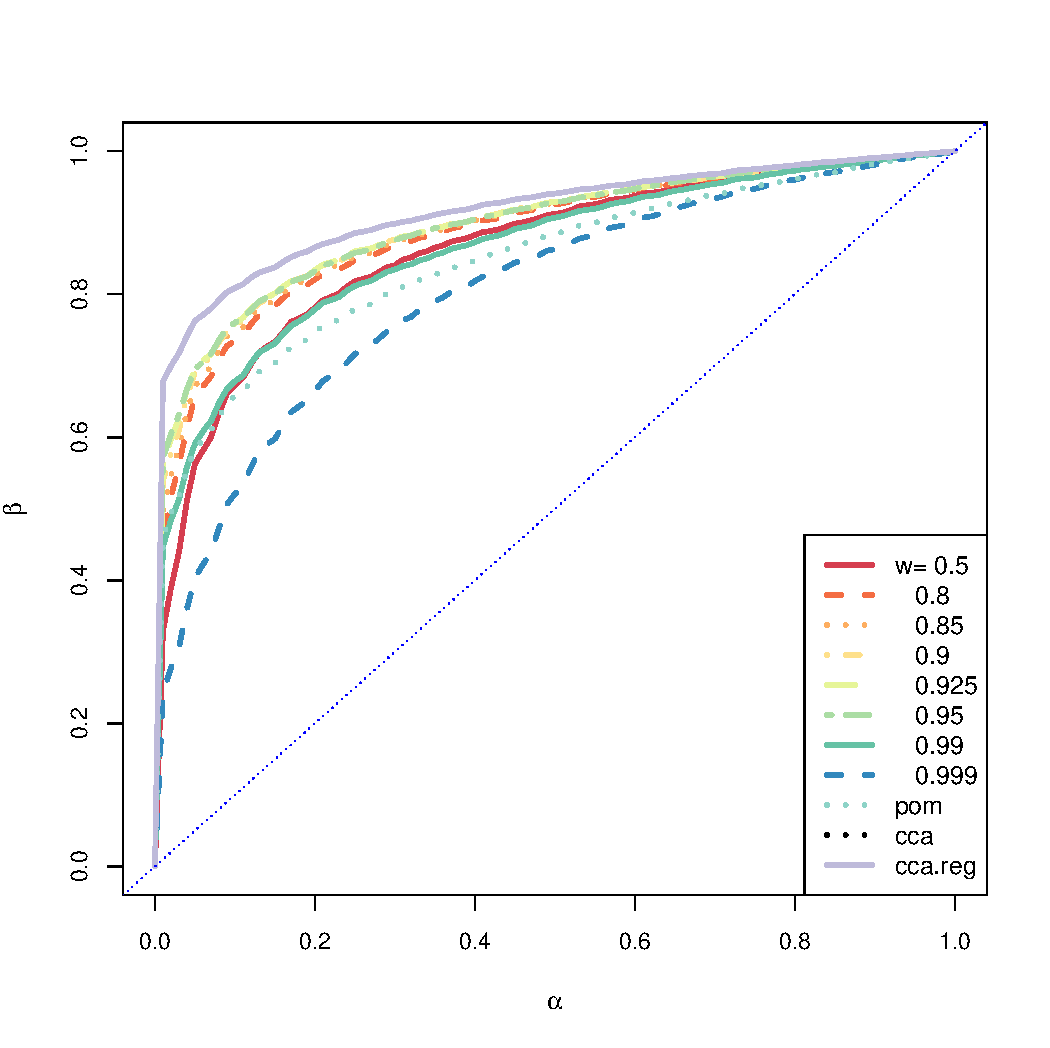
\includegraphics[scale=0.35]{MVN-FC-Tradeoff-OOS-c0.pdf}
\caption{Power ($\beta$) vs Type I error ($\alpha$) plot for different $w$ values for the Gaussian setting}
\label{fig:MVN-c0-power-alpha}
        \end{subfigure}%        
         \begin{subfigure}[b]{0.45\textwidth}  
         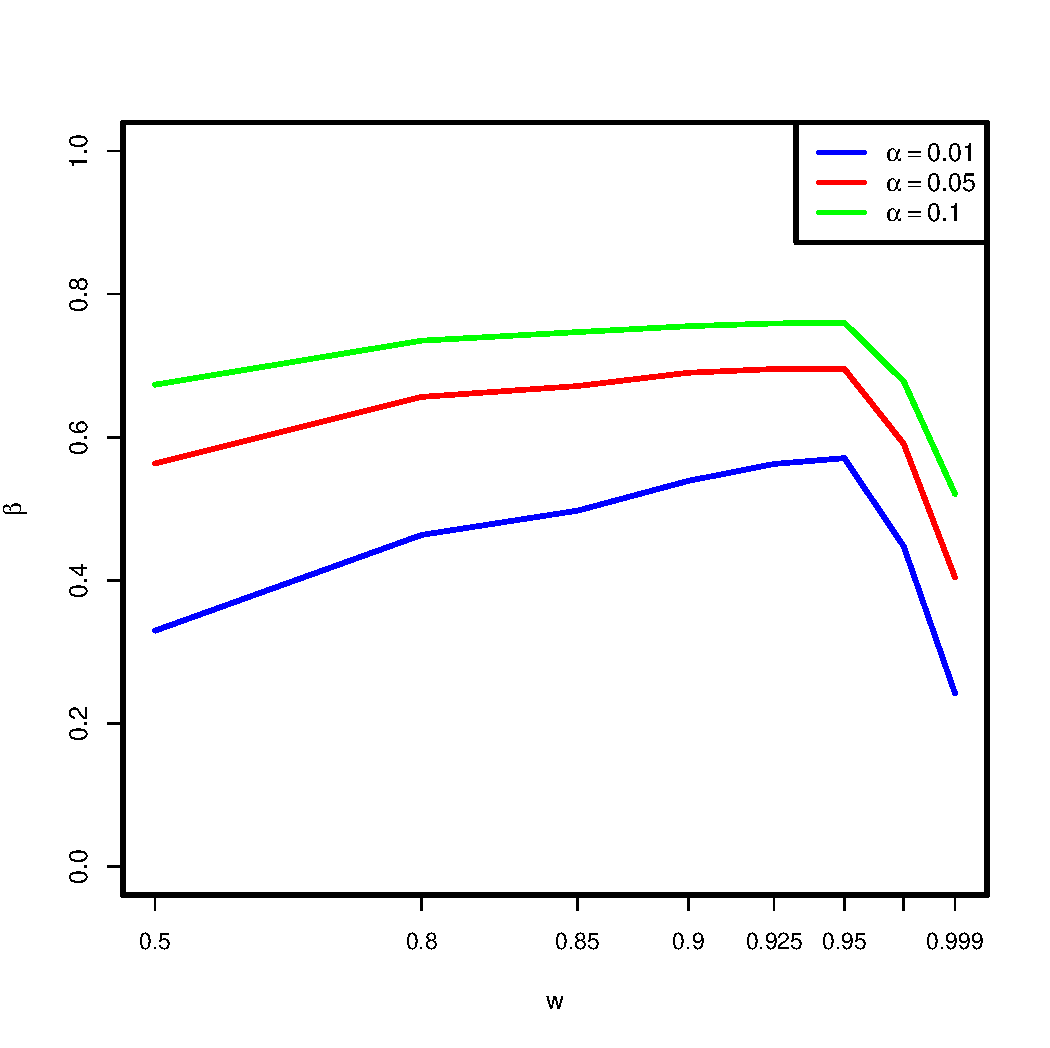
\includegraphics[scale=0.95]{OOSMVN-power-w-c0.pdf}
\caption{Power ($\beta$) vs $w$ plot for different Type I error ($\alpha$) values for the Gaussian setting}
\label{fig:MVN-c001-power-w}
         \end{subfigure}%
          
  \caption {ROC curves and $\beta$ vs $w$ plots for simulation experiments}
  \end{figure}


Setting p and q to 5 and 10, respectively, for $n=150$ matched training pairs and $m=150$ matched and unmatched test pairs, the average of the power values for $nmc=150$ Monte Carlo replicates are computed at  different $\alpha$s and are plotted in Figure \ref{fig:MVN-c001-power-w} against $\alpha$ for the Gaussian setting.  Qualititatively similar plots for the Dirichlet setting  are not included for brevity.  The plot in Figure \ref{fig:MVN-c001-power-w} shows that for different values of  $w$, $\beta$-$\alpha$ curves vary significantly.  The conclusion is that the match detection tests with JOFC embedding using specific $w$ values have better performance than other $w$ values in terms of power.  In Figure
 \ref{fig:MVN-c001-power-w},  $\beta(w)$ is plotted against $w$ for fixed values of $\alpha$. It is  interesting that the optimal value of $w$ seems to be in the range of $(0.85,1)$ for this setting, which suggests a significant emphasis on commensurability might be  critical for the match detection  task. Simulations with other paramater values  resulted in $w^*$ estimates closer to $0.5$.




\begin{comment}
\begin{figure}
\includegraphics[scale=0.35]{OOS-MVN-power-w-c0.pdf}
\caption{$\beta$ vs $w$ plot for fixed $\alpha$ values for the Gaussian setting (noiseless case)}
\label{fig:MVN-c0-beta-w}
\end{figure}


\begin{figure}
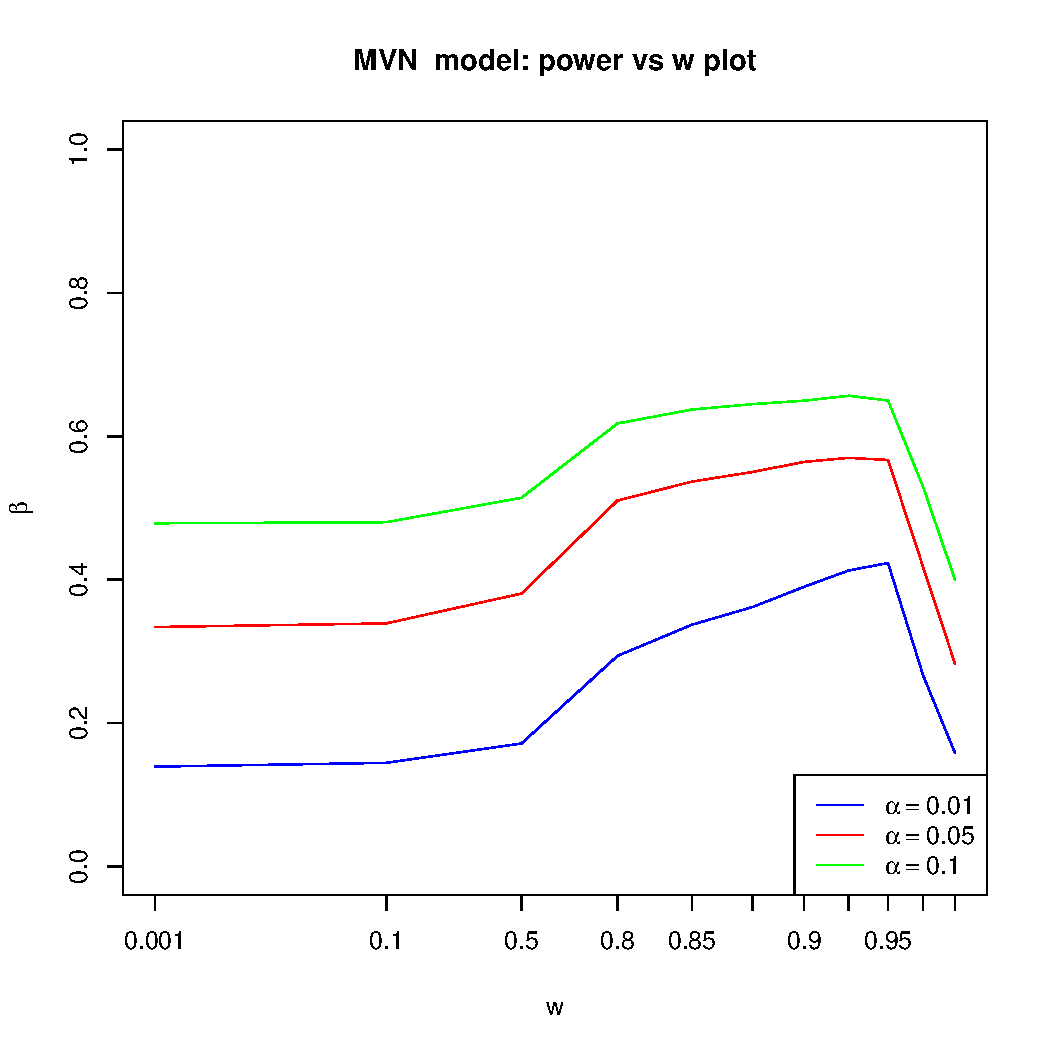
\includegraphics[scale=0.65]{OOSMVN-power-w-c001.pdf}
\caption{Power ($\beta$) vs $w$ plot for fixed Type I error ($\alpha$) values for the Gaussian setting (noisy case)}
\label{fig:MVN-c001-beta-w}
\end{figure}

\end{comment}

Note that in Figure \ref{fig:MVN-c001-power-w} for $\alpha=0.05$, $\beta_{\alpha=0.05}(w=0.99)\geq\beta_{\alpha=0.05}(w=0.5)$. However, for $\alpha=0.3$, $\beta_{\alpha=0.3}(w=0.99)\leq\beta_{\alpha=0.3}(w=0.5)$. This justifies our comment that  $w^{*}$  must be defined with respect to $\alpha$.


\begin{comment}
\begin{figure}
\includegraphics[scale=0.35]{OOS-Dirichlet-power-w-c0.pdf}
\caption{$\beta$ vs $w$ plot for fixed $\alpha$ values for the Dirichlet setting(noiseless case)}
\label{fig:fig7}
\end{figure}

\begin{figure}
\includegraphics[scale=0.35]{OOS-Dirichlet-power-w-c0-01.pdf}
\caption{$\beta$ vs $w$ plot for fixed $\alpha$ values for the Dirichlet setting(noisy case)}
\label{fig:fig8}
\end{figure}
\end{comment}



Note that  for all of the settings, the estimate of the optimal $w^{*}$ has  higher power than $w$=0.5 (the unweighted case).

\begin{comment}



\section{Model Selection}
For the simulations presented up to now, the embedding dimension $d$ was set to 2. This was a convenient choice which allowed us to investigate various aspects of JOFC and competing approaches.
However,  more care is required in selection of this parameter, since it plays such a big role in performance in general learning settings. The signal dimension was set to $p=10$ and different $d=2,5,7,10,15$ values were used to test the JOFC approach.
The following plots of ROC curves in    \ref{fig:ROC-d} and  \ref{fig:ROC-d-15} shows the effect of $d$ parameter on the performance of different methods for the Gaussian setting for the noisy case. 
\begin{figure}
 \centering
  \captionsetup[subfigure]{labelformat=empty}
        \begin{subfigure}[b]{0.5\textwidth}        
               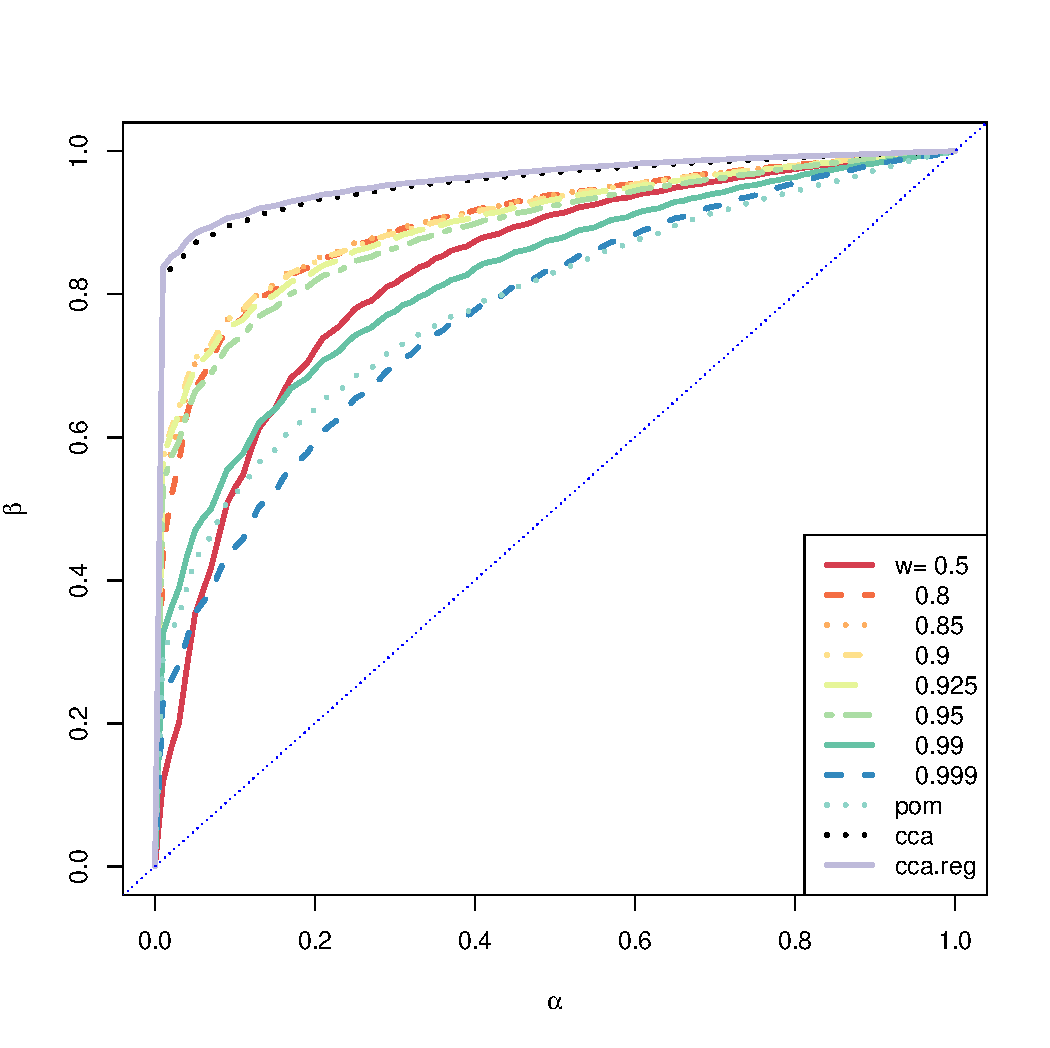
\includegraphics[width=\textwidth]{ROC-d-2.pdf}
                \caption{d=2}
                \label{fig:ROC-d-2}
        \end{subfigure}%
         %add desired spacing between images, e. g. ~, \quad, \qquad etc. 
          %(or a blank line to force the subfigure onto a new line)
        \begin{subfigure}[b]{0.5\textwidth}           
                  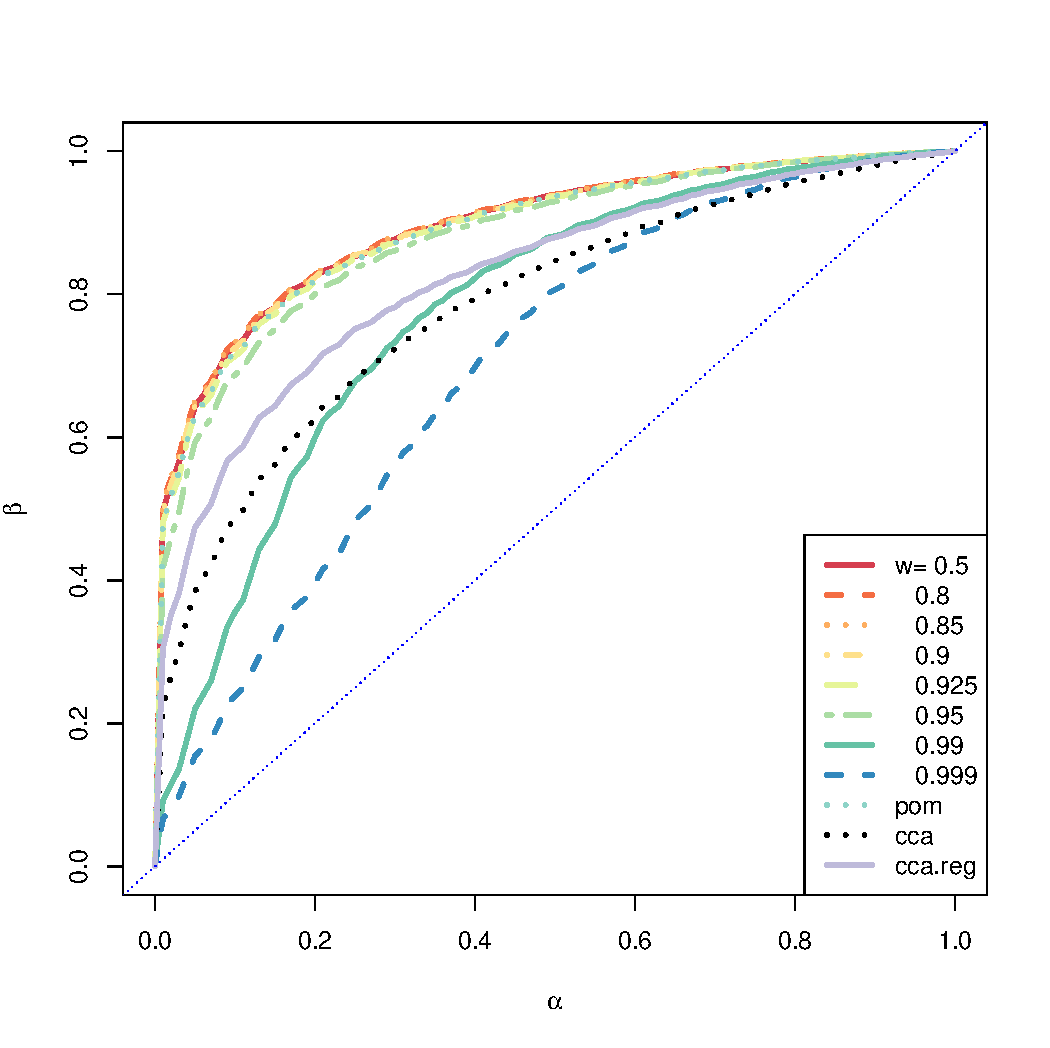
\includegraphics[width=\textwidth]{ROC-d-5.pdf}
                \caption{d=5}
                \label{fig:ROC-d-5}
        \end{subfigure}      
        %add desired spacing between images, e. g. ~, \quad, \qquad etc.    %(or a blank line to force the subfigure onto a new line)
        \begin{subfigure}[b]{0.47\textwidth}             
               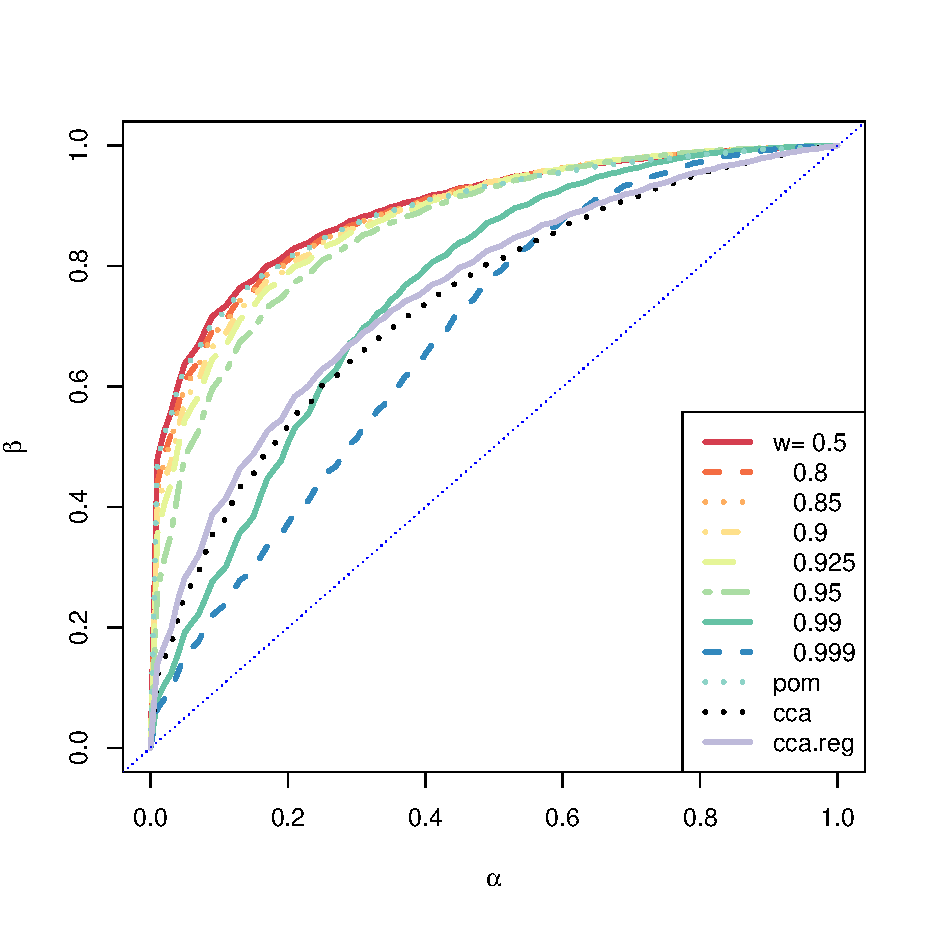
\includegraphics[width=\textwidth]{ROC-d-7.pdf}
                \caption{d=7}
                \label{fig:ROC-d-7}
        \end{subfigure}          
               \begin{subfigure}[b]{0.47\textwidth}
                \centering
               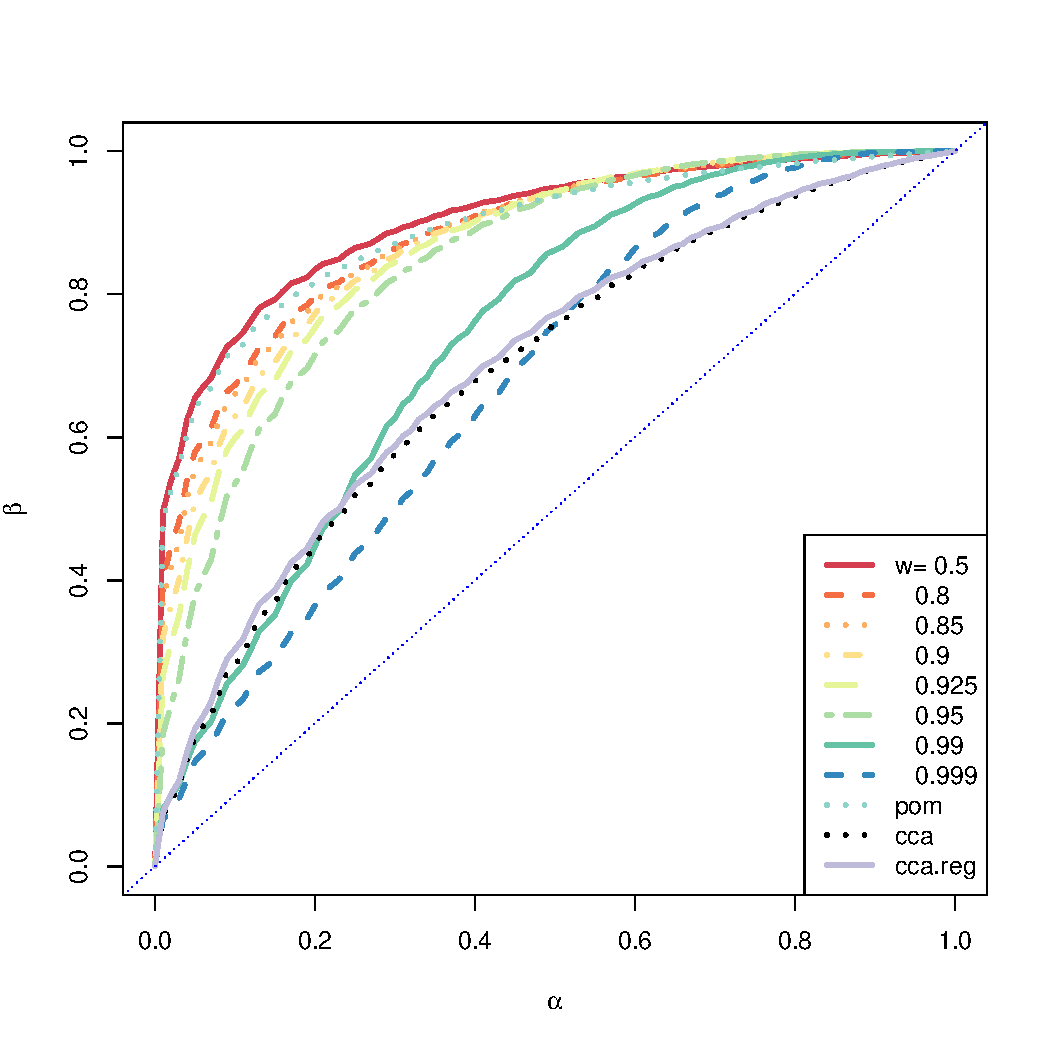
\includegraphics[width=\textwidth]{ROC-d-10.pdf}
                \caption{d=10}
                \label{fig:ROC-d-10}
        \end{subfigure}
        
          \begin{subfigure}[b]{0.47\textwidth}
             \centering
               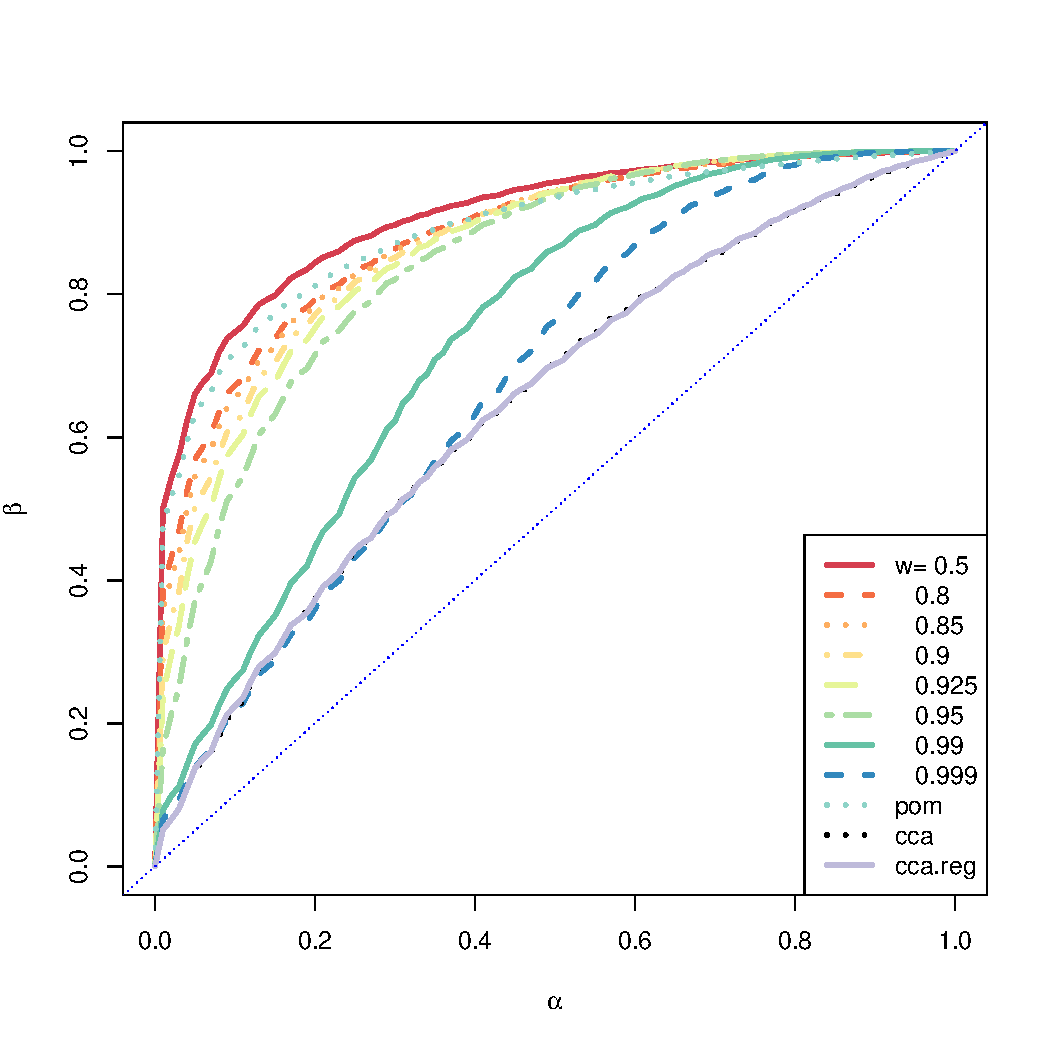
\includegraphics[scale=0.3]{ROC-d-15.pdf}
                \caption{d=15}
                \label{fig:ROC-d-15}
                        \end{subfigure}
         
        \caption{Effect of $d$ parameter on ROC plots}\label{fig:ROC-d}
        \label{fig:ROC-d}

\end{figure}


\end{comment}

\section{Conclusion}
 The tradeoff between Fidelity and Commensurability and the relation to the weighted raw stress criterion for MDS were both investigated with several simulations and experiments on real data.
   For  hypothesis testing as the exploitation task, the three approaches were compared in terms of testing power.
    The results indicate that when doing a joint optimization, one should consider an optimal compromise point between Fidelity and Commensurability,
       which corresponds to an optimal weight $w^*$ of the weighted raw stress criterion in contrast to the unweighted raw stress 
        for omnibus matrix embedding. 
        


\bibliographystyle{plain}
\bibliography{priebe-thesis-JOFC}



\end{document}
